\documentclass[tikz,border=12pt]{standalone}
\usepackage{amsmath,amssymb}
\usepackage{tikz}
\usetikzlibrary{arrows.meta,decorations.pathreplacing,calc}

\definecolor{fineC}{HTML}{1F4E79}
\definecolor{coarseC}{HTML}{B45309}
\definecolor{envC}{HTML}{0B6E4F}
\definecolor{ink}{HTML}{1A1A1A}
\definecolor{bgSoft}{HTML}{F7F5F1}
\definecolor{gridLite}{HTML}{D1D5DB}

\begin{document}
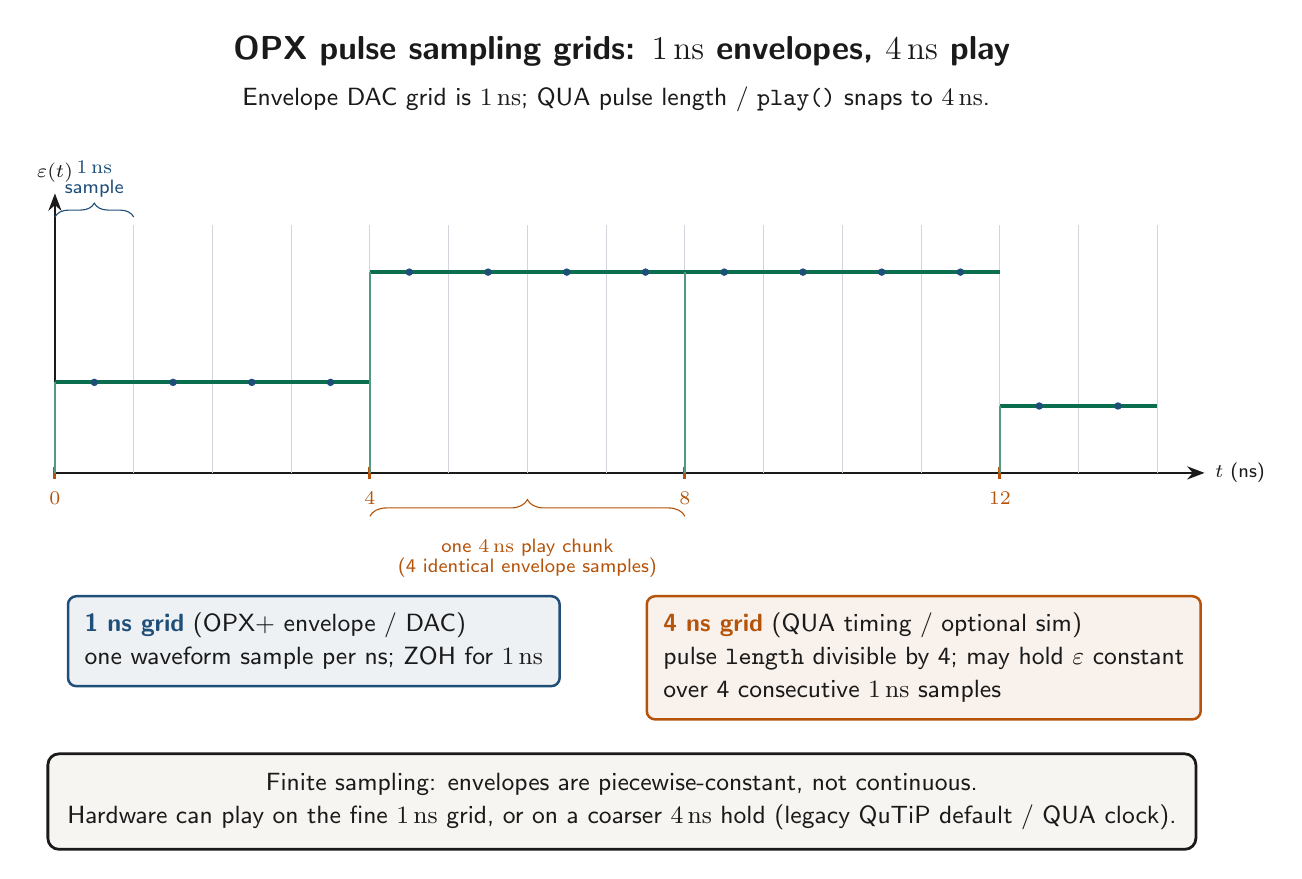
\begin{tikzpicture}[
  font=\sffamily\small,
  >={Stealth[length=2.2mm]},
  title/.style={font=\sffamily\bfseries\large, text=ink}
]

\node[title] at (7.2,5.35) {OPX pulse sampling grids: $1\,\mathrm{ns}$ envelopes, $4\,\mathrm{ns}$ play};
\node[align=center, text=ink] at (7.2,4.75) {%
  Envelope DAC grid is $1\,\mathrm{ns}$; QUA pulse length / \texttt{play()} snaps to $4\,\mathrm{ns}$.
};

% axes
\draw[->, line width=1pt, ink] (0,0) -- (14.6,0) node[right, font=\sffamily\scriptsize] {$t$ (ns)};
\draw[->, line width=1pt, ink] (0,0) -- (0,3.55) node[above, font=\sffamily\scriptsize] {$\varepsilon(t)$};

% faint 1 ns vertical grid
\foreach \x in {1,...,14} {
  \draw[line width=0.35pt, gridLite] (\x,0) -- (\x,3.15);
}
% stronger 4 ns ticks
\foreach \x in {0,4,8,12} {
  \draw[line width=1.05pt, coarseC] (\x,-0.08) -- (\x,0.08);
  \node[below, font=\sffamily\scriptsize, text=coarseC] at (\x,-0.12) {$\x$};
}

% piecewise-constant envelope on 1 ns grid (example: 4 ns plateaus = playable on 4 ns)
% heights for samples 0..13 (held), then show rise-ish then flat then fall
% Using 4-ns-constant knobs: same value for 4 consecutive 1 ns samples
\newcommand{\zoh}[3]{% #1=x0, #2=x1, #3=height
  \draw[line width=1.35pt, envC] (#1,#3) -- (#2,#3);
  \draw[line width=0.7pt, envC!70] (#1,0) -- (#1,#3);
}

% rise over first 4 ns (held per ns but drawn as one 4 ns step for clarity of "4 ns play")
\zoh{0}{4}{1.15}
\zoh{4}{8}{2.55}
\zoh{8}{12}{2.55}
\zoh{12}{14}{0.85}

% mark 1 ns sample centers as dots on the flats
\foreach \x/\h in {
  0.5/1.15,1.5/1.15,2.5/1.15,3.5/1.15,
  4.5/2.55,5.5/2.55,6.5/2.55,7.5/2.55,
  8.5/2.55,9.5/2.55,10.5/2.55,11.5/2.55,
  12.5/0.85,13.5/0.85
} {
  \fill[fineC] (\x,\h) circle (1.35pt);
}

% braces: 1 ns vs 4 ns
\draw[decorate, decoration={brace, amplitude=5pt}, fineC]
  (0,3.25) -- (1,3.25);
\node[above, font=\sffamily\scriptsize, text=fineC, align=center] at (0.5,3.38) {%
  $1\,\mathrm{ns}$\\[-1pt] sample
};

\draw[decorate, decoration={brace, amplitude=6pt}, coarseC]
  (4,-0.55) -- (8,-0.55);
\node[below, font=\sffamily\scriptsize, text=coarseC, align=center] at (6,-0.72) {%
  one $4\,\mathrm{ns}$ play chunk\\[-1pt]
  (4 identical envelope samples)
};

% legend boxes
\node[draw=fineC, line width=0.9pt, rounded corners=3pt, fill=fineC!8,
      align=left, inner sep=6pt, text=ink, anchor=north west]
  at (0.15,-1.55) {%
  {\color{fineC}\textbf{1 ns grid}} (OPX+ envelope / DAC)\\[1pt]
  one waveform sample per ns; ZOH for $1\,\mathrm{ns}$
};

\node[draw=coarseC, line width=0.9pt, rounded corners=3pt, fill=coarseC!8,
      align=left, inner sep=6pt, text=ink, anchor=north west]
  at (7.5,-1.55) {%
  {\color{coarseC}\textbf{4 ns grid}} (QUA timing / optional sim)\\[1pt]
  pulse \texttt{length} divisible by 4; may hold $\varepsilon$ constant\\[1pt]
  over 4 consecutive $1\,\mathrm{ns}$ samples
};

\node[draw=ink, line width=1pt, rounded corners=4pt, fill=bgSoft,
      align=center, inner sep=7pt, text=ink, anchor=north]
  at (7.2,-3.55) {%
  Finite sampling: envelopes are piecewise-constant, not continuous.\\[1pt]
  Hardware can play on the fine $1\,\mathrm{ns}$ grid, or on a coarser $4\,\mathrm{ns}$ hold
  (legacy QuTiP default / QUA clock).
};

\end{tikzpicture}
\end{document}
